%\clearpage
\subsubsection{The 1.633 shell-to-core ratio}

The ratio of the axes in an ideally dense hexagonal packing equals $\frac{\sqrt{8}}{3}=1.633$, which became the motivation to use this number as a shell-to-core ratio in the simulations.

No ordered phase was observed for all the considered in this work packing density values in the range from 0.25 to 0.52.%, thus the packing density range was expanded up to the value of 0.55. 
The obtained phase diagram is shown in the \textbf{Figure} \ref{fig:phase_1_63}. The disordered phase in the 0.25-0.51 packing density range is not included. 

\begin{figure}
\centering
\includegraphics[width=0.9\textwidth]{phase1_63.tikz}
\caption{Phase diagram packing density $\eta$ vs shell potential $\epsilon$ at constant $\lambda=1.633$} \label{fig:phase_1_63}
\end{figure}

\begin{figure}[H]
% published
\centering
\begin{subfigure}{.24\textwidth}
  \centering
  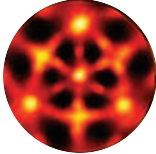
\includegraphics[width=0.95\textwidth]{brass_published}
  \caption{$\gamma$--Brass}
  \label{fig:brass_p} 
\end{subfigure}
\begin{subfigure}{.24\textwidth}
  \centering
   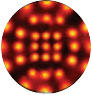
\includegraphics[width=0.95\textwidth]{b_W_published}
  \caption{$\beta$--W}
  \label{fig:betta_w}  
\end{subfigure}
\begin{subfigure}{.24\textwidth}
  \centering
  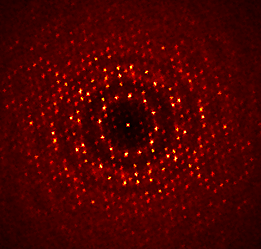
\includegraphics[width=0.95\textwidth]{diff_setpf_53_eps_2}
  \caption{$\eta=0.53,\epsilon=2$}
  \label{fig:diff_xz} 
\end{subfigure}
\begin{subfigure}{.24\textwidth}
  \centering
  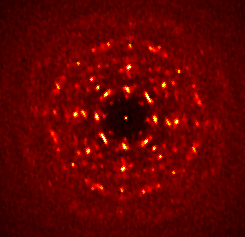
\includegraphics[width=0.95\textwidth]{diffsetpf_0_54_eps_1_00}
  \caption{$\eta=0.54,\epsilon=1$}
  \label{fig:diff_xz2} 
\end{subfigure}
% Found
\begin{subfigure}{.24\textwidth}
  \centering
  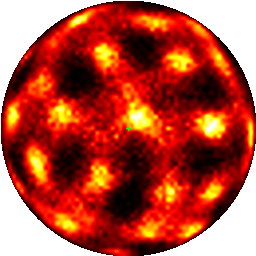
\includegraphics[width=0.95\textwidth]{L_1633_s_0_55_e_2_5}
  \caption{$\eta=0.55,\epsilon=2.5$}
  \label{fig:brass_f} 
\end{subfigure}
\begin{subfigure}{.24\textwidth}
  \centering
   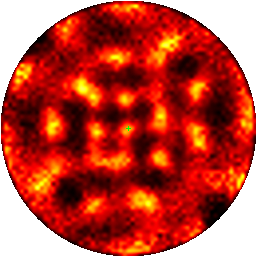
\includegraphics[width=0.95\textwidth]{qc_163_setpf_0_53_eps_1_00}
  \caption{$\eta=0.53,\epsilon=1$}
  \label{fig:betta_w_f}  
\end{subfigure}
\begin{subfigure}{.24\textwidth}
  \centering
  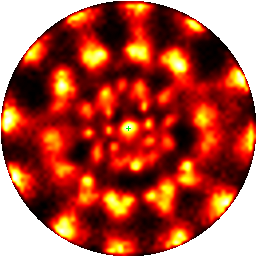
\includegraphics[width=0.95\textwidth]{qc_163_setpf_0_53_eps_2_00}
  \caption{$\eta=0.53,\epsilon=2$}
  \label{fig:bond_xz} 
\end{subfigure}
\begin{subfigure}{.24\textwidth}
  \centering
  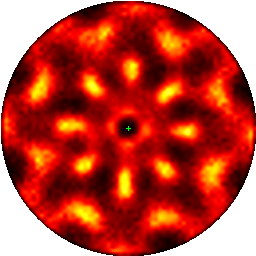
\includegraphics[width=0.95\textwidth]{qc_163_setpf_0_54_eps_1_00}
  \caption{$\eta=0.54,\epsilon=1$}
  \label{fig:bond_xz2} 
\end{subfigure}
\caption{Bond order diagrams and diffraction patterns, observed during simulations at constant $\lambda=1.633$. \subref{fig:brass_p} and \subref{fig:betta_w} -- previously reported bond order diagrams, \subref{fig:diff_xz}, \subref{fig:diff_xz2}, \subref{fig:brass_f}, \subref{fig:betta_w_f}, \subref{fig:bond_xz} and \subref{fig:bond_xz2} -- diffraction patterns and bond order diagrams observed in this work.}
\label{fig:allfrom163}
\end{figure}

At the packing density of 0.55 the diagram is mostly occupied by FCC, however %it seems that 
in very small regions the emergence of QC phase is also possible.
Thus at $\epsilon=2.5$, $\eta=0.55$ and  $\epsilon=1$, $\eta=0.53$  $\gamma$-brass and $\beta$--W phases were observed respectively. Previously reported as well as observed in this work bond order diagrams for the $\gamma$-brass and $\beta$--W phases\cite{engelscience} are shown in the \textbf{Figures} \ref{fig:brass_p}, \ref{fig:brass_f}, \ref{fig:betta_w} and \ref{fig:betta_w_f}.

The bond order diagrams as well as the diffraction patterns of the structures, that were not identified by me in the previously published works are shown in the \textbf{Figures} \ref{fig:diff_xz}, \ref{fig:diff_xz2}, \ref{fig:bond_xz} and \ref{fig:bond_xz2}.
%The structure was obtained in the study of Damasceno et al.\cite{engelscience} during truncated dodecahedra simulations. Another complex structure appears in the region with $\epsilon=1-2$ and $\eta=0.53-0.54$. The structure is apparently a 12-fold QC.





